% \textbf{\underline{OZ 2 - Magnetische velden - Oefening 1:}}
% \vspace{0.5cm}

% Het circuit op Figuur 2.1 bestaat uit draden aan de boven- en onderkant van twee identieke metalen veren aan de linker- en rechterzijde. De bovenkant van het circuit staat vast. De draad aan de onderkant heeft een massa van $ 10.0 g $ en is $ 5.00 cm $ lang. De veren rekken $ 0.500 cm $ uit onder het gewicht van de draad en het circuit heeft een totale weerstand van $ 12.0 \Omega $. Wanneer een magnetisch veld wordt aangelegd dat uit het blad wijst, rekken de veren een extra $ 0.300 cm $ uit. Wat is de grootte van het magnetische veld?

% \begin{figure}[H]
%     \centering
%     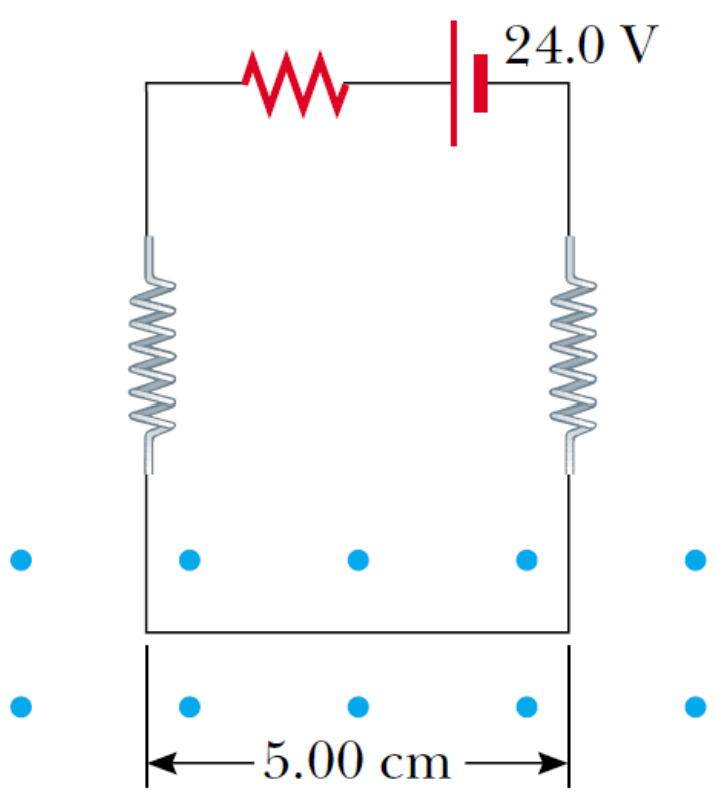
\includegraphics[width=5.5cm]{oz02/resources/oef-1-opgave.png}
    
%     \textbf{Figuur 2.1}
% \end{figure}

% \begin{description}[labelwidth=1.5cm, leftmargin=!]
%     \item[Geg. :]   $ m = 10,0 $ g; $ s = 5,00 $ cm; $ x_0 = 0,500 $ cm; $ R = 12,0 \ \Omega $; $ \Delta x_e = 0,300 $ cm; $ V = 24,0 $ V;
%     \item[Gevr. :]  $ \left| \left| \vec{B} \right| \right| $;
%     \item[Opl. :]   $ I = \dfrac{V}{R} = \dfrac{24,0}{12,0} = 2 $ A
    
%                     \vspace{0.3 cm}
    
%                     $ \sum F_y = 0 $
                    
%                     \hspace{-0.57 cm} $ \Leftrightarrow 
%                     2 F_V - F_G = 0 $
                    
%                     \hspace{-0.57 cm} $ \Leftrightarrow
%                     F_V = \dfrac{F_G}{2}
%                     = \dfrac{m \cdot g}{2}
%                     = \dfrac{10,0 \cdot 10^{-3} \cdot 9,81}{2}
%                     = 0,04905 $ N
    
%                     \vspace{0.3 cm}
                    
%                     $ F_V = k \cdot x_0 $
                    
%                     \hspace{-0.57 cm} $ \Leftrightarrow 
%                     k = \dfrac{F_V}{x_0}
%                     = \dfrac{0,0495}{0,500 \cdot 10^{-2}}
%                     = 9,81 $ N/m
    
%                     \vspace{0.3 cm}
                    
%                     $ \sum F_y = 0 $ 
                    
%                     \hspace{-0.57 cm} $ \Leftrightarrow
%                     2 F_V - F_G - F_M = 0 $
                    
%                     \hspace{-0.57 cm} $ \Leftrightarrow
%                     F_M = 2 F_V - F_G
%                     = 2 \cdot k \cdot (x_0 + \Delta x_e) - m \cdot g $
                    
%                     \hspace{0.54 cm} $
%                     = 2 \cdot 9,81 \cdot (0,500 \cdot 10^{-2} + 0,300 \cdot 10^{-2}) - 10,0 \cdot 10^{-3} \cdot 9,81
%                     = 0,05886 $ N
    
%                     \vspace{0.3 cm}
                    
%                     $ d\vec{F} = I d\vec{s} \times \vec{B} $
                    
%                     \hspace{-0.57 cm} $ \Rightarrow
%                     \left| \left| \vec{F_M} \right| \right| = I \cdot \left| \left| \vec{s} \right| \right| \cdot \left| \left| \vec{B} \right| \right| \cdot \sin{90^{\circ}} $
                    
%                     \hspace{-0.57 cm} $ \Leftrightarrow
%                     \left| \left| \vec{B} \right| \right| = \dfrac{\left| \left| \vec{F_M} \right| \right|}{I \cdot \left| \left| \vec{s} \right| \right| \cdot \sin{90^{\circ}}}
%                     = \dfrac{0,05886}{2 \cdot 5,00 \cdot 10^-2 \cdot \sin{90^\circ}}
%                     = 0,5886 $ T $
%                     \approx 0,589 $ T
% \end{description}

% \vspace{1cm}